\documentclass[11pt]{article}
\usepackage{fancyhdr}
\usepackage{tocloft}
\usepackage{graphicx}
\usepackage{calc}
\usepackage{amssymb}
\usepackage{color}
\usepackage[sc]{mathpazo}
\usepackage{url}
\usepackage{ifpdf}
\usepackage{bbding}
\usepackage{caption}
\usepackage{framed}
\usepackage{xcolor}
\usepackage{float}
\usepackage{wrapfig}
\usepackage{sidecap}
\linespread{1.0}
\oddsidemargin=0pt
\evensidemargin=0pt
\textwidth=6.5in
\topmargin=0pt
\headheight=0pt
\headsep=0pt
\textheight=9in
\setlength{\parindent}{0.25cm}
\newcommand\secfont{\fontfamily{cmss}\selectfont}%\textwidth 5.5truein
\newcommand\pifheading[1]{\noindent{\secfont\textbf{#1}:}}
\newcommand\yr{2016}
\def\lo{
\mathrel{\raise.3ex\hbox{$<$}\mkern-14mu\lower0.6ex\hbox{$\sim$}}
}
\def\hi{
\mathrel{\raise.3ex\hbox{$>$}\mkern-14mu\lower0.6ex\hbox{$\sim$}}
}

\textwidth = 6.5 in
\textheight = 9 in
\oddsidemargin = -0.00 in
\evensidemargin = +0.05 in
\topmargin = 0 in
\headheight = 0.0 in
\headsep = 0.0 in
\parskip = 0.05in

\newcommand\registered{{\ooalign{\hfil\raise .00ex\hbox{\scriptsize R}\hfil\crcr\mathhexbox20D}}}

%% Define a new 'leo' style for the package that will use a smaller font.
\makeatletter
\def\url@leostyle{%
  \@ifundefined{selectfont}{\def\UrlFont{\sf}}{\def\UrlFont{\small\ttfamily}}}
\makeatother
%% Now actually use the newly defined style.
\urlstyle{leostyle}
\newcommand\checkme[1]{\textcolor{blue}{\textbf{#1}}}
\newcounter{hours}\newcounter{minutes}
\newcommand\printtime{\setcounter{hours}{\time/60}\setcounter{minutes}{\time - \value{hours}*60}\thehours :\theminutes}
\newenvironment{packed_item}{
\begin{itemize}
 \setlength{\itemsep}{1pt}
 \setlength{\parskip}{0pt}
 \setlength{\parsep}{0pt}
}{\end{itemize}}

\newenvironment{packed_enum}{
\begin{enumerate}
 \setlength{\itemsep}{1pt}
 \setlength{\parskip}{0pt}
 \setlength{\parsep}{0pt}
}{\end{enumerate}}

\newenvironment{box_list}{
\begin{itemize}
 \setlength{\itemsep}{3pt}
 \setlength{\parskip}{0pt}
 \setlength{\parsep}{0pt}
}{\end{itemize}}

\newenvironment{packed_list}{
\begin{list}{\labelitemi}{\leftmargin=1em}
 \setlength{\itemsep}{3pt}
 \setlength{\parskip}{0pt}
 \setlength{\parsep}{0pt}
}{\end{list}}

\renewenvironment{quote}{%
  \list{}{%
    \leftmargin10pt   % this is the adjusting screw
    \rightmargin\leftmargin
  }
  \item\relax
}
{\endlist}

% definition of a new float type (refer to the caption package documentation)
\DeclareCaptionType{boxcaption}[Box]
\captionsetup[boxcaption]{position=top,labelfont=bf}

% definition of a shaded-like environment (see framed.sty)
\newenvironment{shadedframe}
  {\def\FrameCommand{\setlength\fboxsep{10pt}\fcolorbox{black}{shadecolor}}%
    \MakeFramed {\advance\hsize-\width \FrameRestore}}%
{\endMakeFramed}

\newenvironment{shadedbox}{%
  \def\FrameCommand{\colorbox{shadecolor}}%
  \MakeFramed {\FrameRestore}}%
 {\endMakeFramed}

% main environment
% syntax: \begin{myenv}{placement-specifiers}{color}{width}...\end{myenv}
\newenvironment{boxenv}[3]
  {\colorlet{shadecolor}{#2}%
    \begin{boxcaption}[#1]%
    \noindent\begin{minipage}{#3}
      \begin{shadedframe}
      }
  {\end{shadedframe}\end{minipage}\end{boxcaption}}

 % TOC
\usepackage{enumerate}
\begin{document}


\begin{figure}
  
\includegraphics[width=\linewidth/3]{title}
  \label{fig:title}
\end{figure}


\title{Lab Report 5: The Diode Basic Properties and Circuits}


\author{Yuezhe Yao}

%\institute{Syracuse University}



\maketitle

\begin{abstract}
In the first part of the lab, we built two VIs to measure, store and analyze the IV characteristics of two common types of diodes: a rectifier diode and a Zener diode.  In the second half of the lab, we built a new VI that essentially operates as a two channel digital oscilloscope, and then you used this VI to observe and characterize the properties of several basic, but important, diode circuits, including the half wave rectifier and the diode clipper.       
\end{abstract}

\medskip

\begingroup
\let\clearpage\relax
\tableofcontents
\endgroup

\medskip
\medskip

\section{Learning Objectives}



To gain additional experience in the use of LabVIEW to configure and operate your DAQ for analog input operations. This will include learning how to trigger your AI operation off of an externally applied TTL signal.

To learn how to use LabVIEW to analyze data with a least-squares fitting function.

To become familiar with the properties and operation of two common types of diodes.

To gain additional experience constructing circuits on the 503 proto-typing board.

\section{Activity I - Measuring the Current Voltage (IV) Characteristics of the 1N4007 Diode}

\begin{figure}[H]
 \begin{center}
  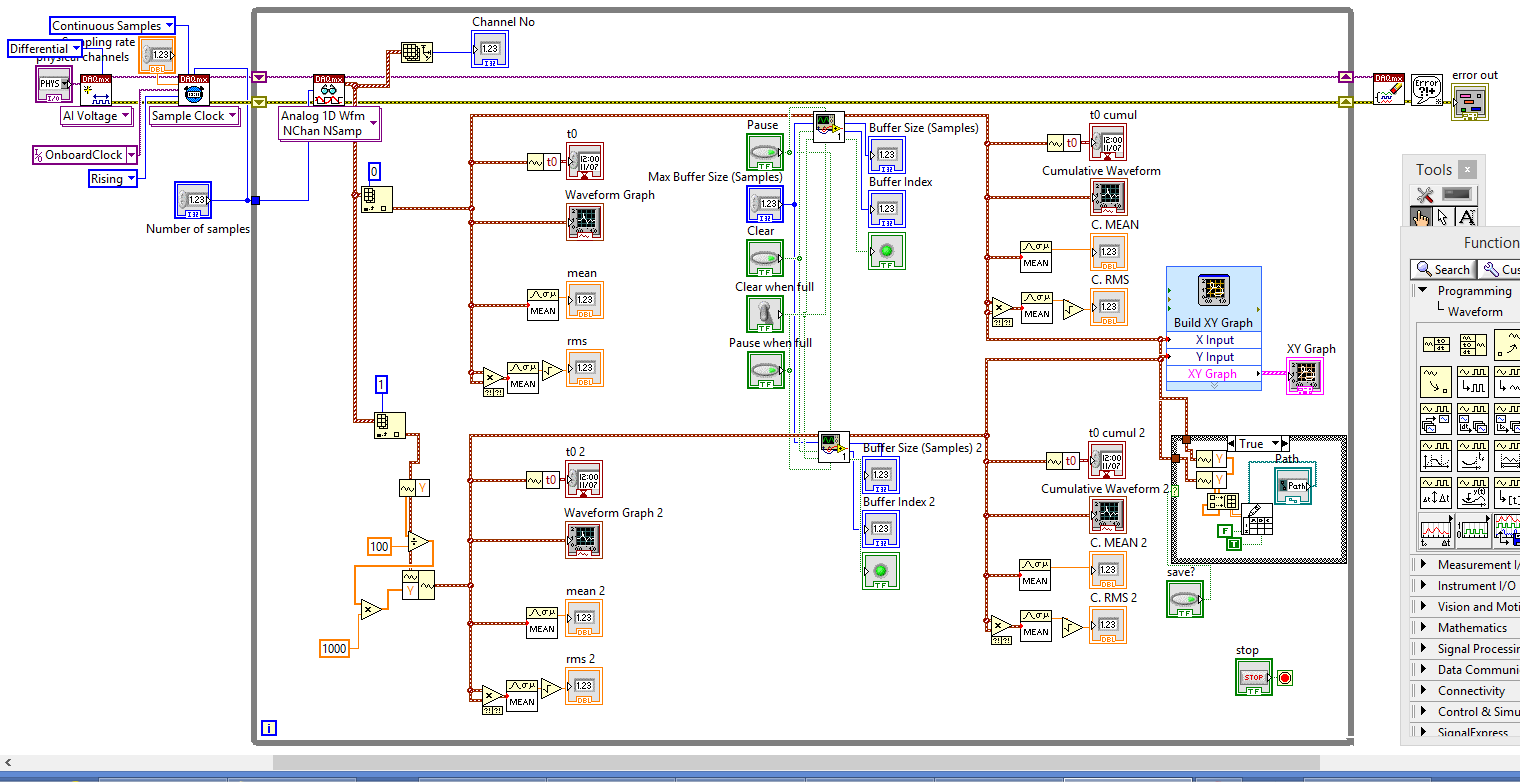
\includegraphics[width=\linewidth/1]{act1bp}
  \caption{The block diagram of the VI.}
  \label{fig:act1bp}
 \end{center}
\end{figure}

\begin{figure}[H]
 \begin{center}
  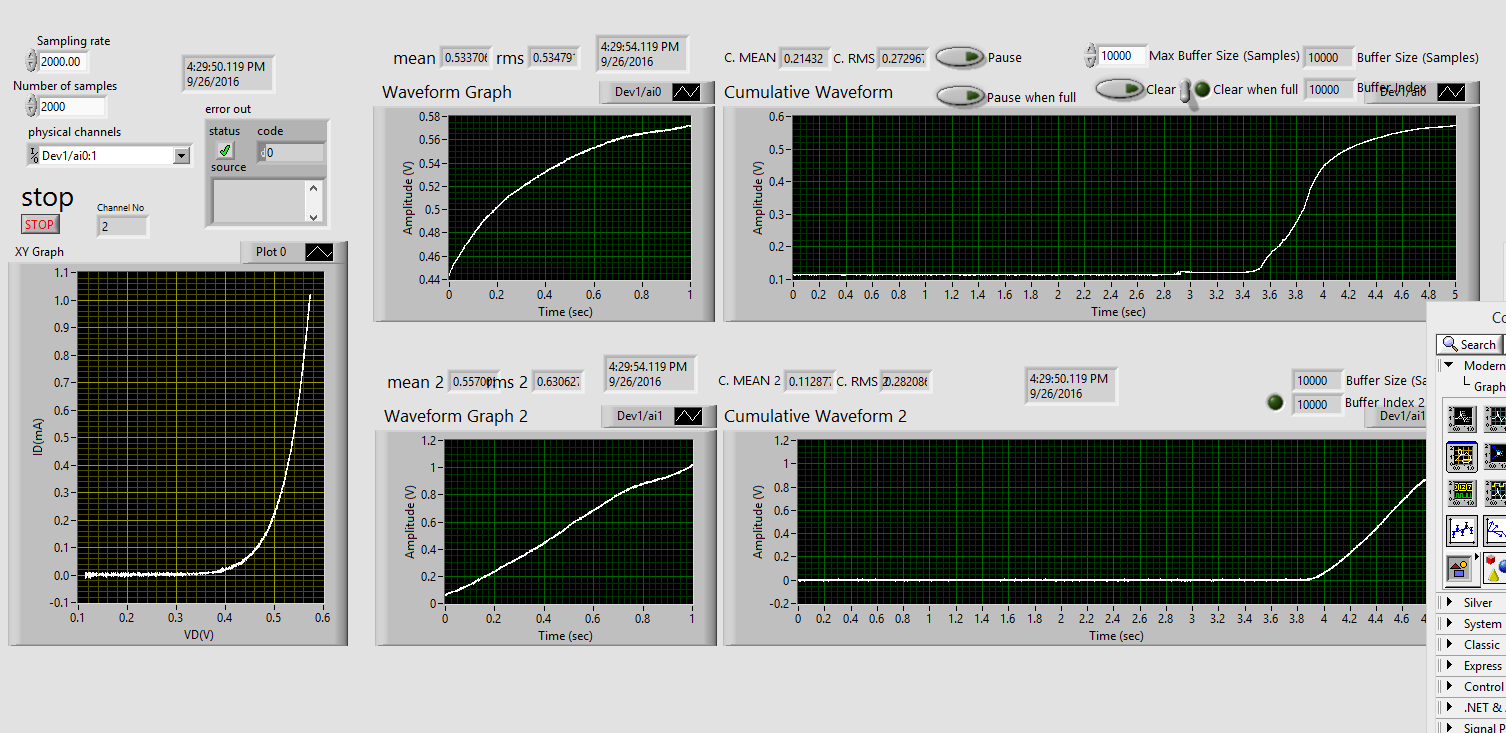
\includegraphics[width=\linewidth/1]{act1bias}
  \caption{The front panel image for forward bias IV measurements.}
  \label{fig:act1bias}
 \end{center}
\end{figure}

\begin{figure}[H]
 \begin{center}
  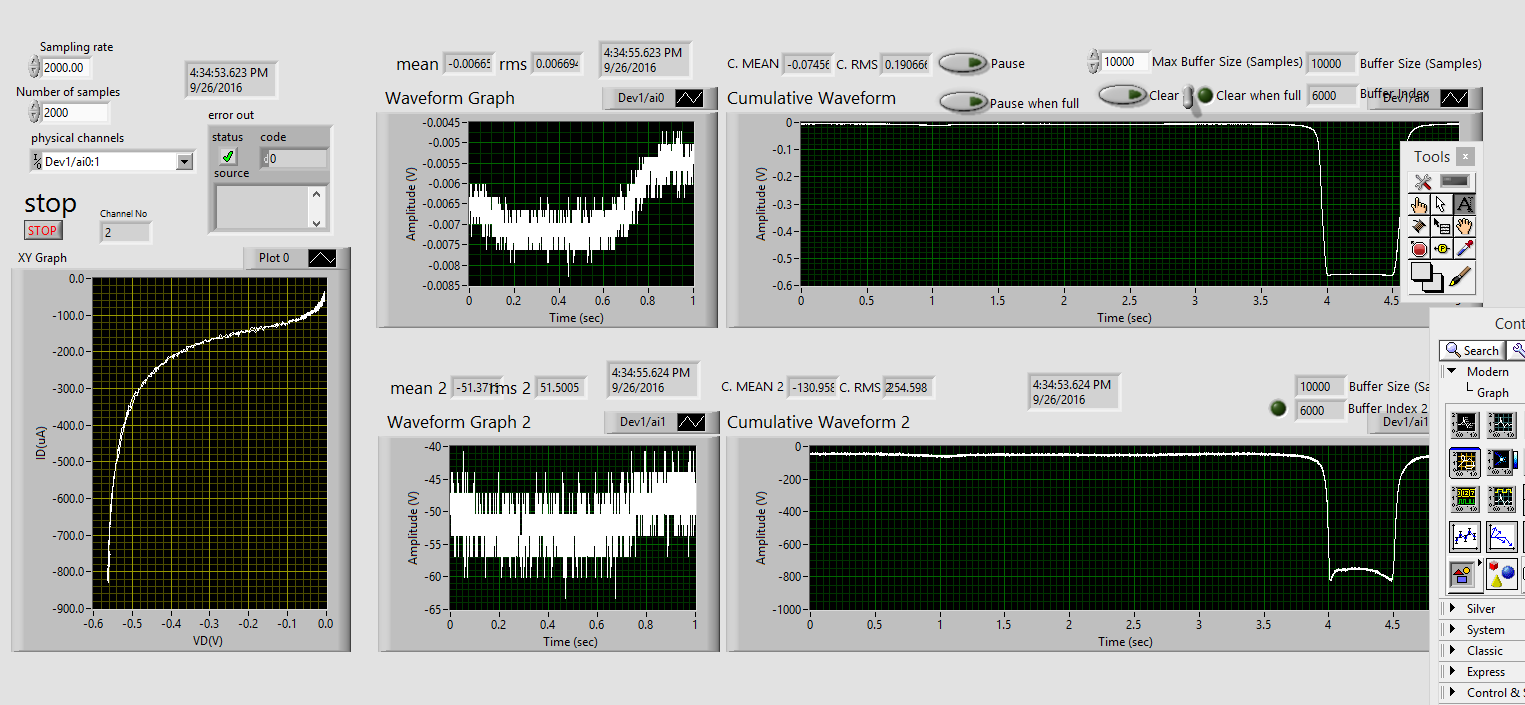
\includegraphics[width=\linewidth/1]{act1rev2}
  \caption{The front panel image for reverse bias IV measurements.}
  \label{fig:act1rev2}
 \end{center}
\end{figure}

$V_{\mathrm {s} }=5 V$

$V_{\mathrm {Dmax} }=0.58 V$

$I_{\mathrm {Dmax} }=1 mA$

$R_{\mathrm {3} }=100 \Omega$

$R_{\mathrm {2} }=470 \Omega$

$R_{\mathrm {1} }=4700 \Omega$

$\Rightarrow V_{\mathrm {R2} }=I_{\mathrm {Dmax} }*R_{\mathrm {3} }+V_{\mathrm {Dmax} }=0.1+0.58=0.68 V$

$\Rightarrow I_{\mathrm {R2} }={\frac {V_{\mathrm {R2} }}{R_{\mathrm {2} }}}=0.68/470=1.447 mA $

$\Rightarrow I_{\mathrm {total} }=I_{\mathrm {R2} }+I_{\mathrm {Dmax} }=1.447+1=2.447 mA $

$\Rightarrow P_{\mathrm {smax} }=I_{\mathrm {total} }*V_{\mathrm {s} }=0.002447*5=0.012 w $ \\[1em]

$ V_{\mathrm {R1} }=V_{\mathrm {s} }-V_{\mathrm {R2} }=5-0.68=4.32 V $

$\Rightarrow P_{\mathrm {R1} }=I_{\mathrm {total} }*V_{\mathrm {R1} }=0.002447*4.32=0.0106 w $ \\[1em]

$\Rightarrow P_{\mathrm {R2} }=I_{\mathrm {R2} }*V_{\mathrm {R2} }=0.001447*0.68=0.984 mw $ \\[1em]

$P_{\mathrm {R3} }=I_{\mathrm {D} }^2*R_{\mathrm {3} }=0.001^2*100=0.1 mw $

From the pictures, we can see that our knee voltage is around 0.45V, which is consistent with what we have read for the diode (0.7V$\sim{Silicon}$, 0.3V$\sim{Germanium}$). And the reverse saturation current is around 200 $\mu$ A, which we think is too large compared to what we expect.



\section{Activity II - Fitting Your IV Measurements to the Shockley Diode Equation Using a LabVIEW Least-Squares Fitting Function}


\begin{figure}[H]
 \begin{center}
  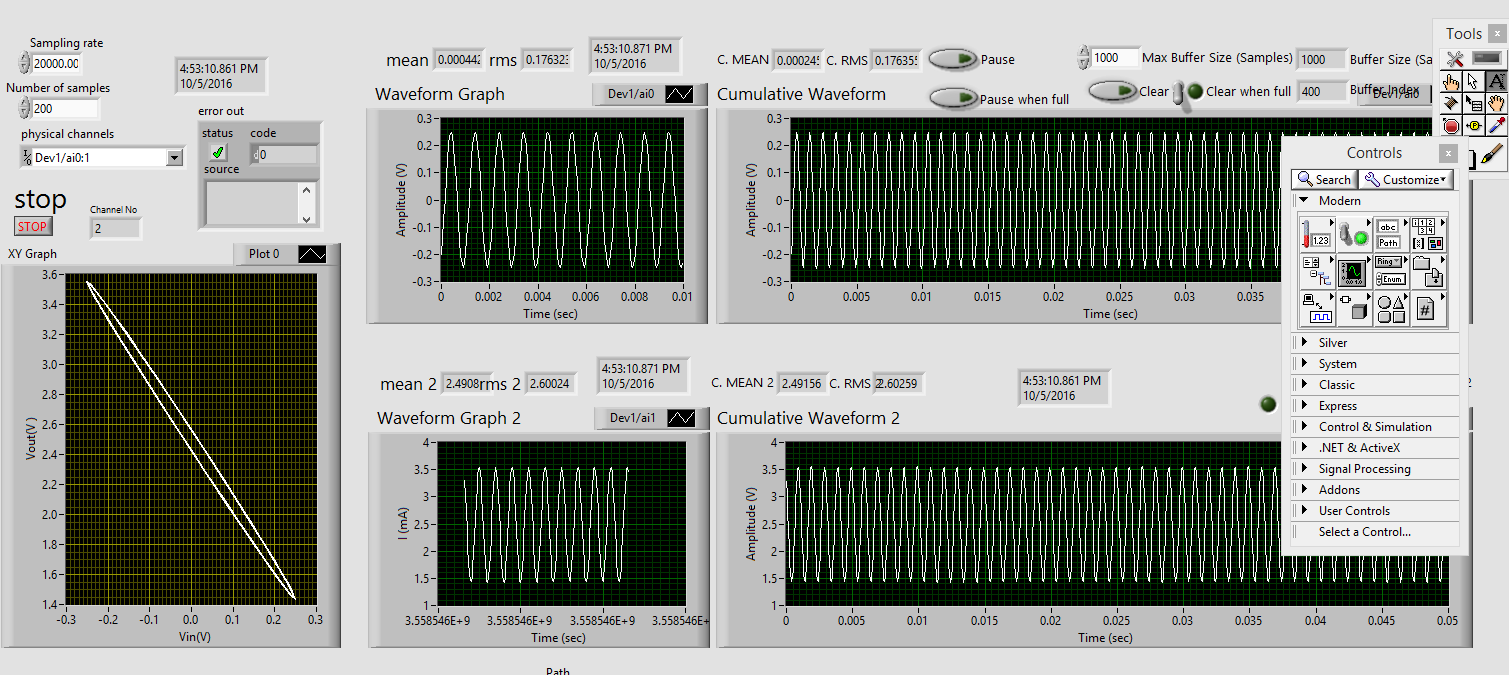
\includegraphics[width=\linewidth/1]{act2}
  \caption{The the front panel and block diagram for our fitting VI.}
  \label{fig:act2}
 \end{center}
\end{figure}

The unit of the y axis in this picture should be mA, we forgot to modify it. And our fitting equation is $y=a*(e^{bx}-1)$, so if we compare that to $I_{\mathrm {D} }=I_{\mathrm {s} }*(e^{V_{\mathrm {D} }/ \eta V_{\mathrm {T} }}-1)$, we'll find that $I_{\mathrm {s} }=a=3.4 nA$ and $\eta=1/{bV_{\mathrm {T} }}=1/{21.92*0.026}=1.75$, which is consistent with what we expect($ \eta \approx 2$ and $I_{\mathrm {s} }\sim 1-5 nA$).

PS: $T=300k$

$V_{\mathrm {T} }=k_{\mathrm {B} }T/e=1.38064852*10^{-23}*300/(1.6*10^{-19})=0.026$



\section{Activity III - Measuring the Characteristics of the 1N4735A Zener Diode}



\begin{figure}[H]
 \begin{center}
  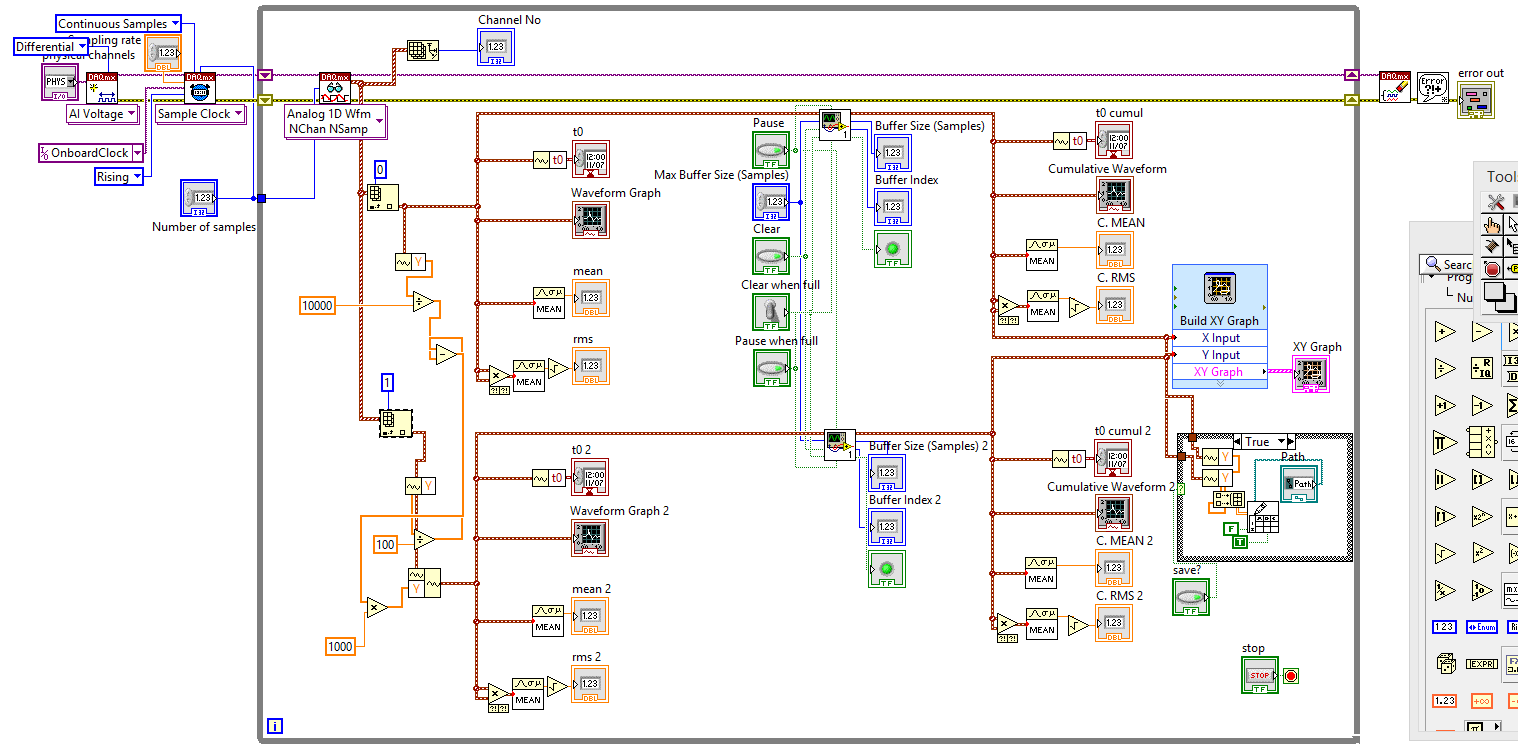
\includegraphics[width=\linewidth/1]{act3bp}
  \caption{The block diagram of the VI.}
  \label{fig:act3bp}
 \end{center}
\end{figure}

\begin{figure}[H]
 \begin{center}
  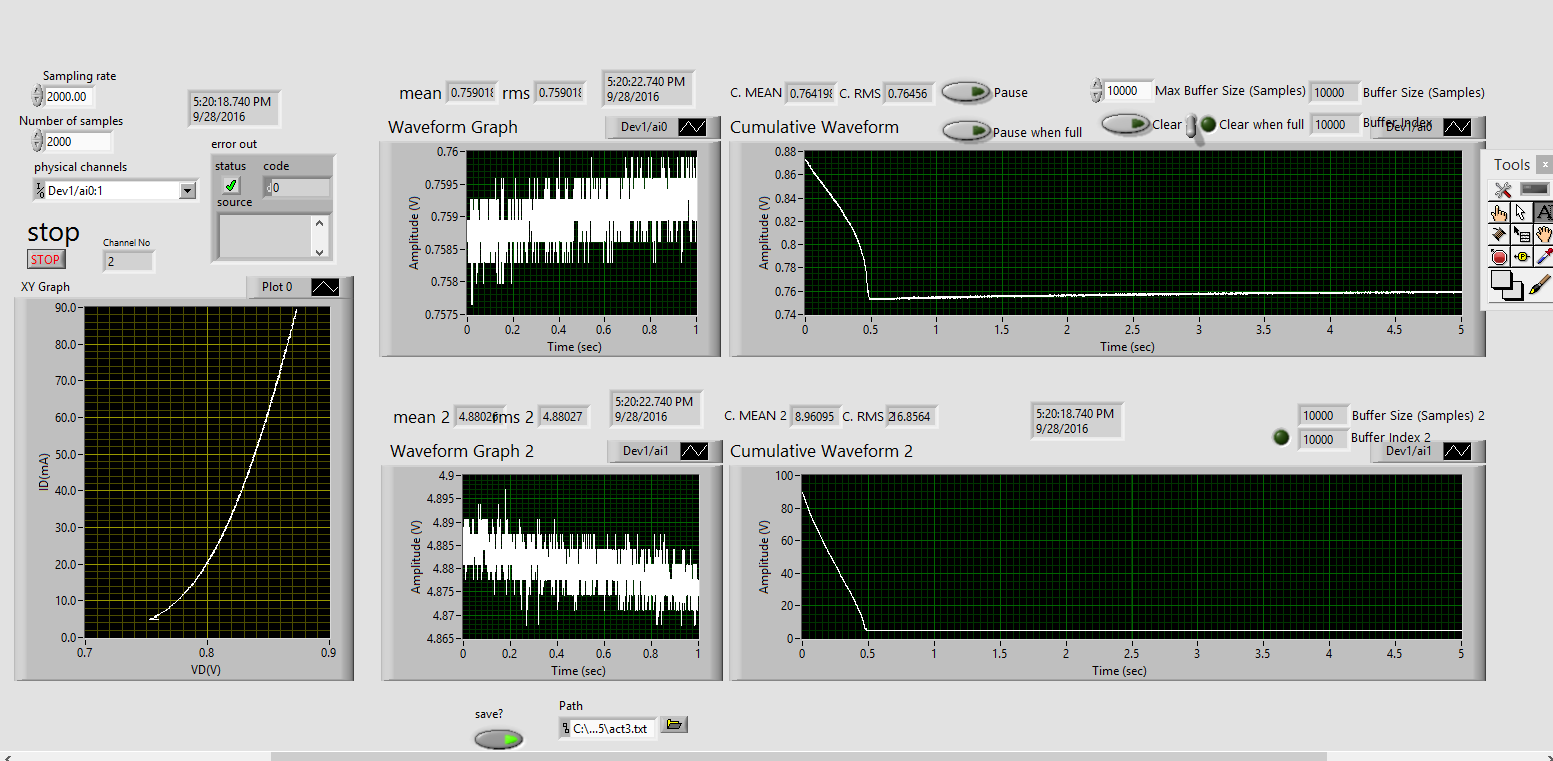
\includegraphics[width=\linewidth/1]{act3bias2}
  \caption{The front panel of the forward bias IV measurements.}
  \label{fig:act3bias2}
 \end{center}
\end{figure}

\begin{figure}[H]
 \begin{center}
  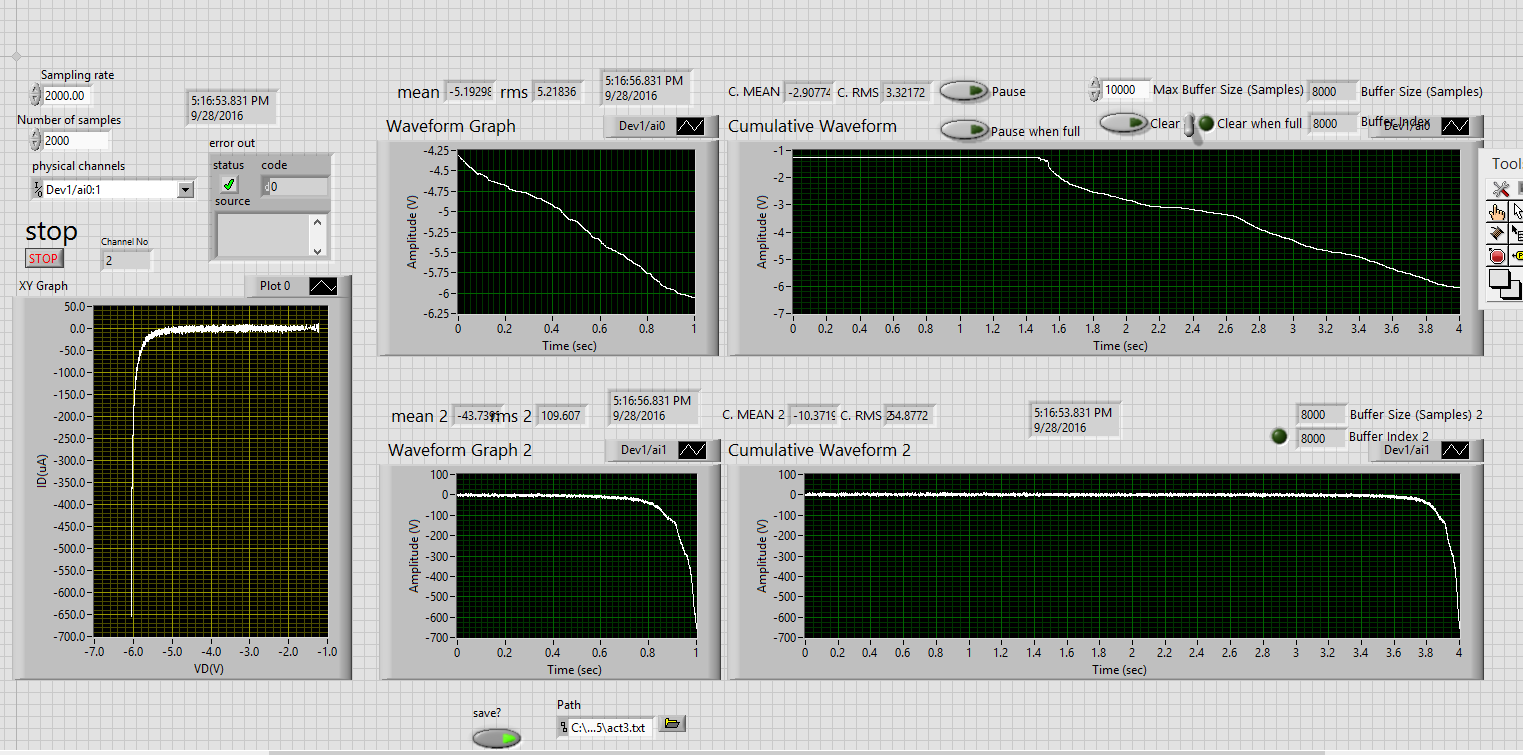
\includegraphics[width=\linewidth/1]{act3rev1}
  \caption{The front panel of the reverse bias IV measurements.}
  \label{fig:act3rev1}
 \end{center}
\end{figure}

\begin{figure}[H]
 \begin{center}
  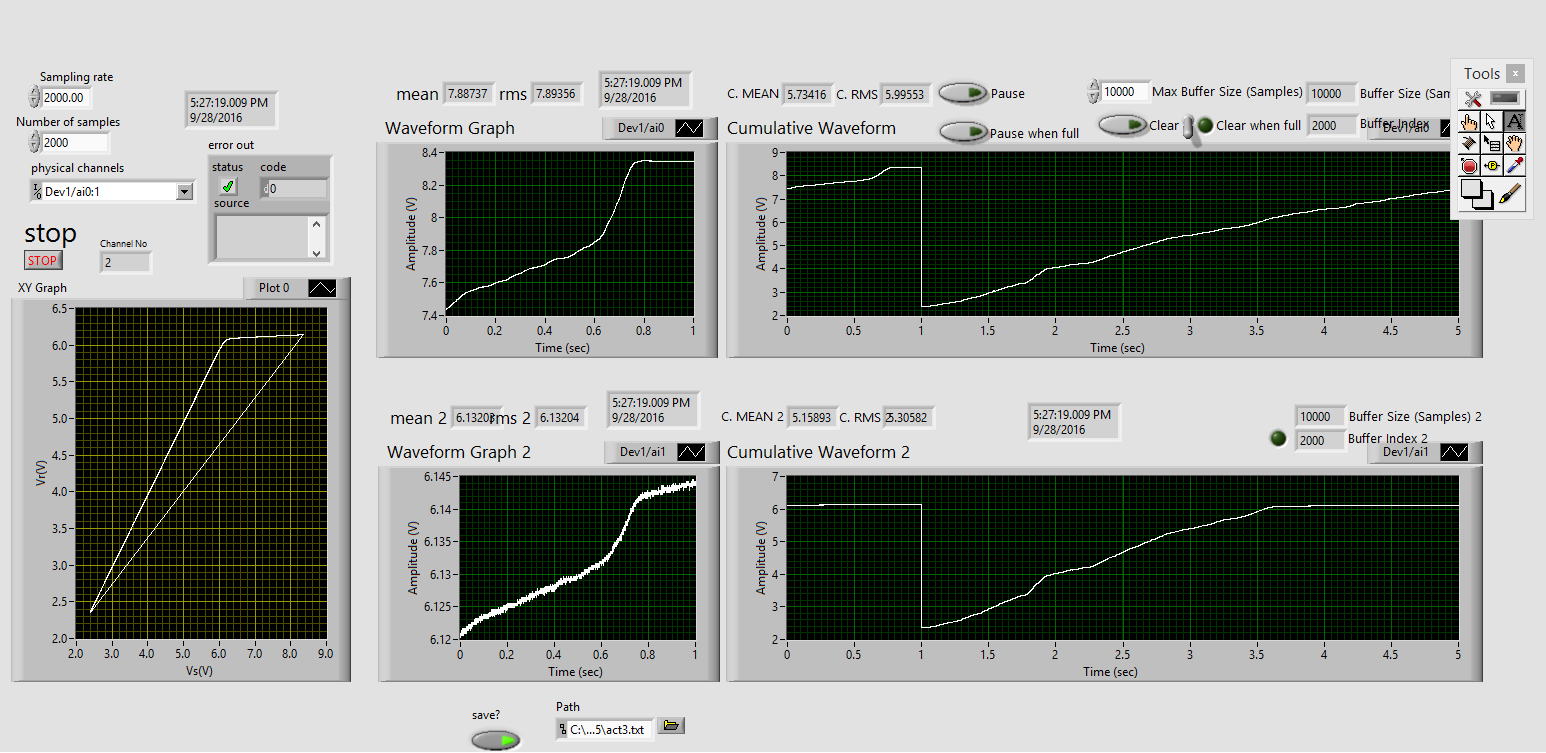
\includegraphics[width=\linewidth/1]{act3vv}
  \caption{The image of the data for the voltage regulation circuit.}
  \label{fig:act3vv}
 \end{center}
\end{figure}

\section{Activity V - Building and Characterizing Some Important Diode-Based Circuits}

\begin{figure}[H]
 \begin{center}
  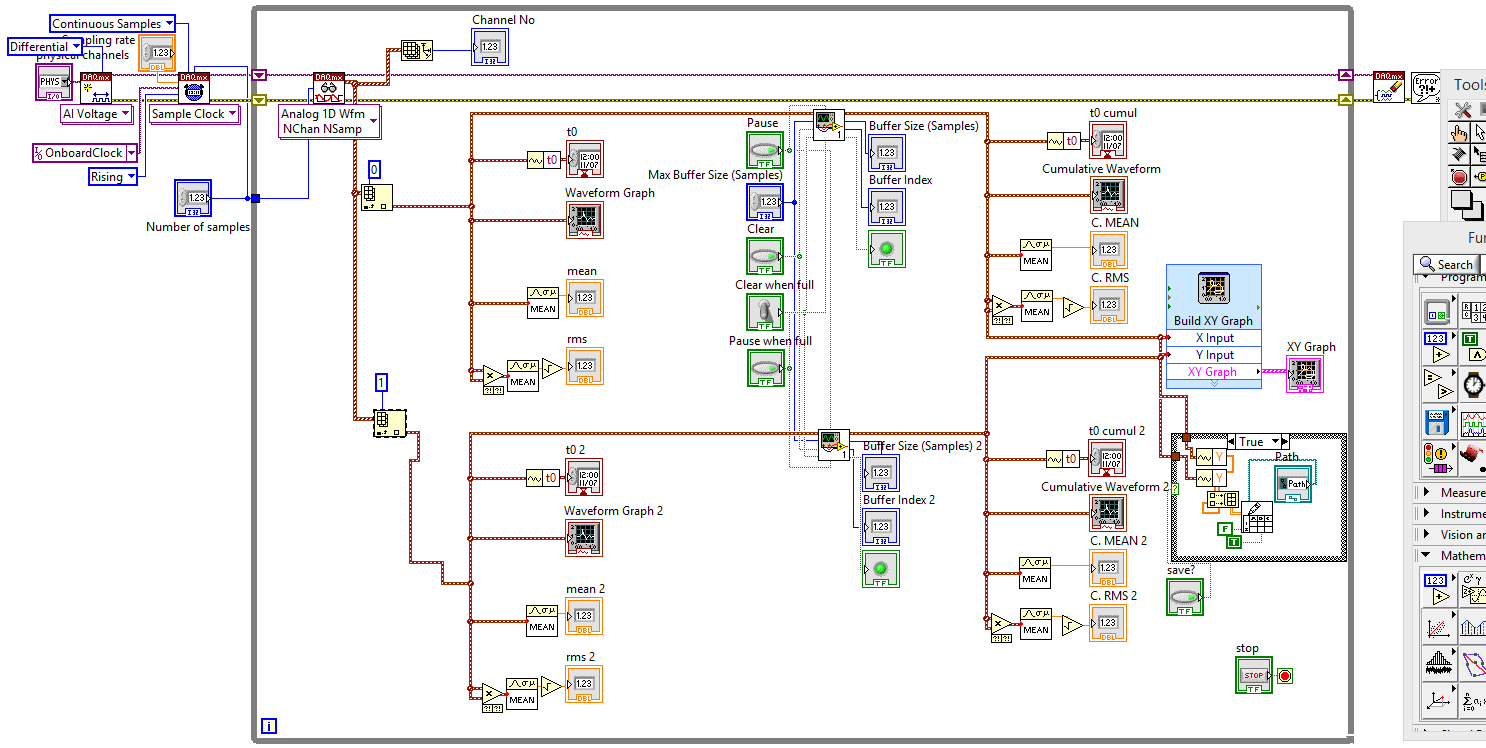
\includegraphics[width=\linewidth/1]{act5bp}
  \caption{The block diagram of the VI.}
  \label{fig:act3bp}
 \end{center}
\end{figure}

\begin{figure}[H]
 \begin{center}
  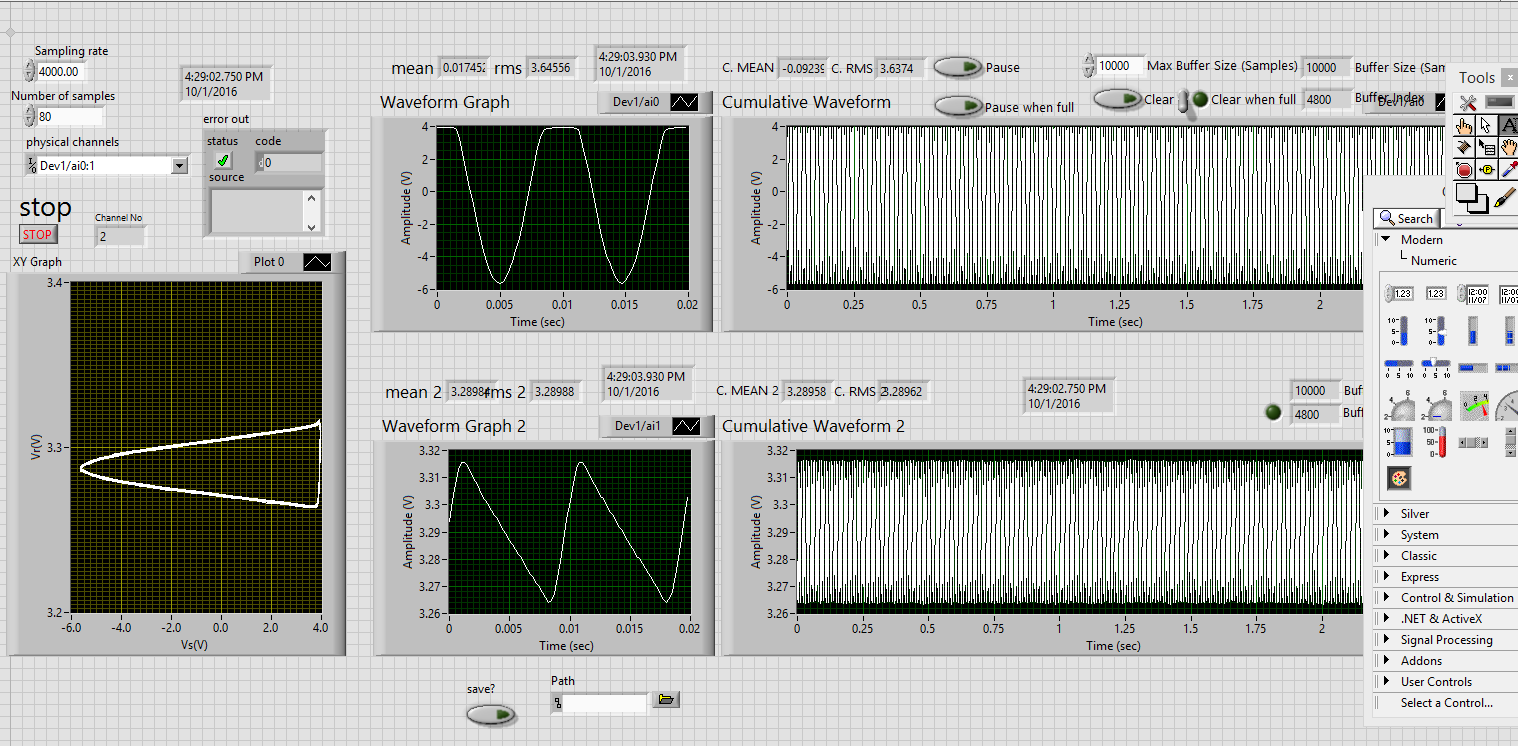
\includegraphics[width=\linewidth/1]{act5acapac100Hz}
  \caption{The front panel of the half-wave rectifier with the capacitor(100Hz).}
  \label{fig:act5acapac100Hz}
 \end{center}
\end{figure}

\begin{figure}[H]
 \begin{center}
  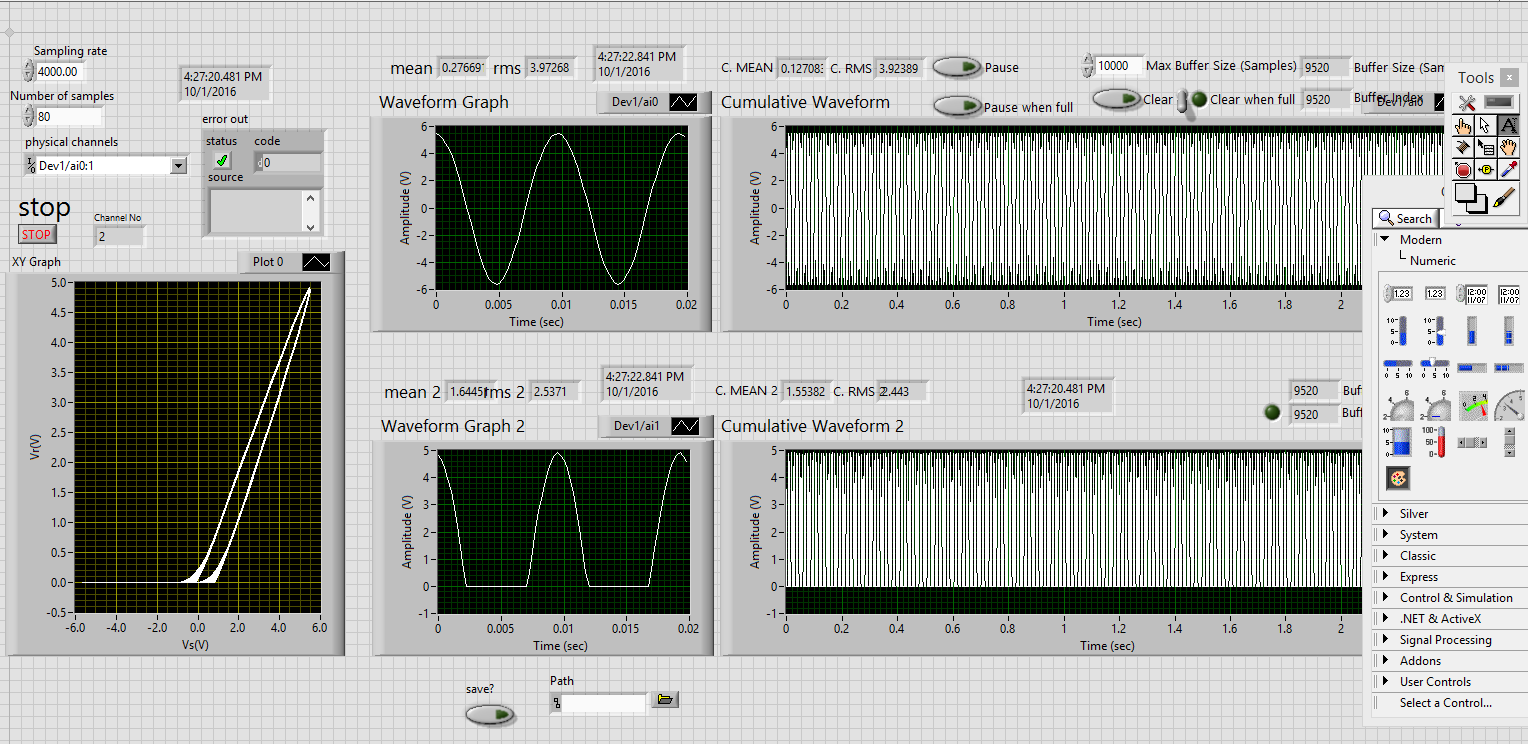
\includegraphics[width=\linewidth/1]{act5anocapac100Hz}
  \caption{The front panel of the half-wave rectifier without the capacitor(100Hz).}
  \label{fig:act5anocapac100Hz}
 \end{center}
\end{figure}

\begin{figure}[H]
 \begin{center}
  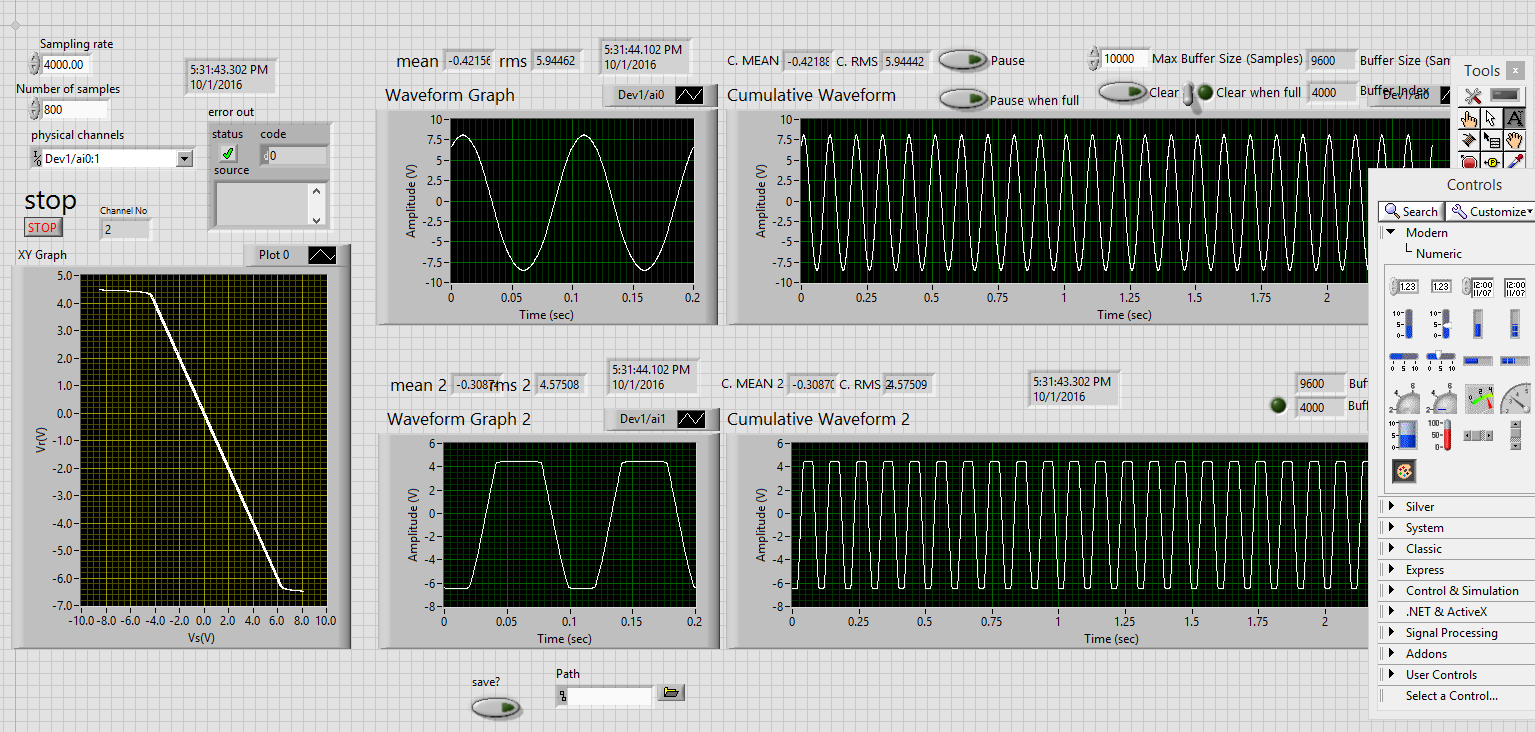
\includegraphics[width=\linewidth/1]{act5b10Hz4v-6v}
  \caption{The front panel of the diode clipper(V1=4V, V2=-6V).}
  \label{fig:act5b10Hz4v-6v}
 \end{center}
\end{figure}

\begin{figure}[H]
 \begin{center}
  \includegraphics[width=\linewidth/1]{act5c10Hzcapac}
  \caption{The front panel of the full-wave rectifier with the capacitor(10Hz).}
  \label{fig:act5c10Hzcapac}
 \end{center}
\end{figure}

\begin{figure}[H]
 \begin{center}
  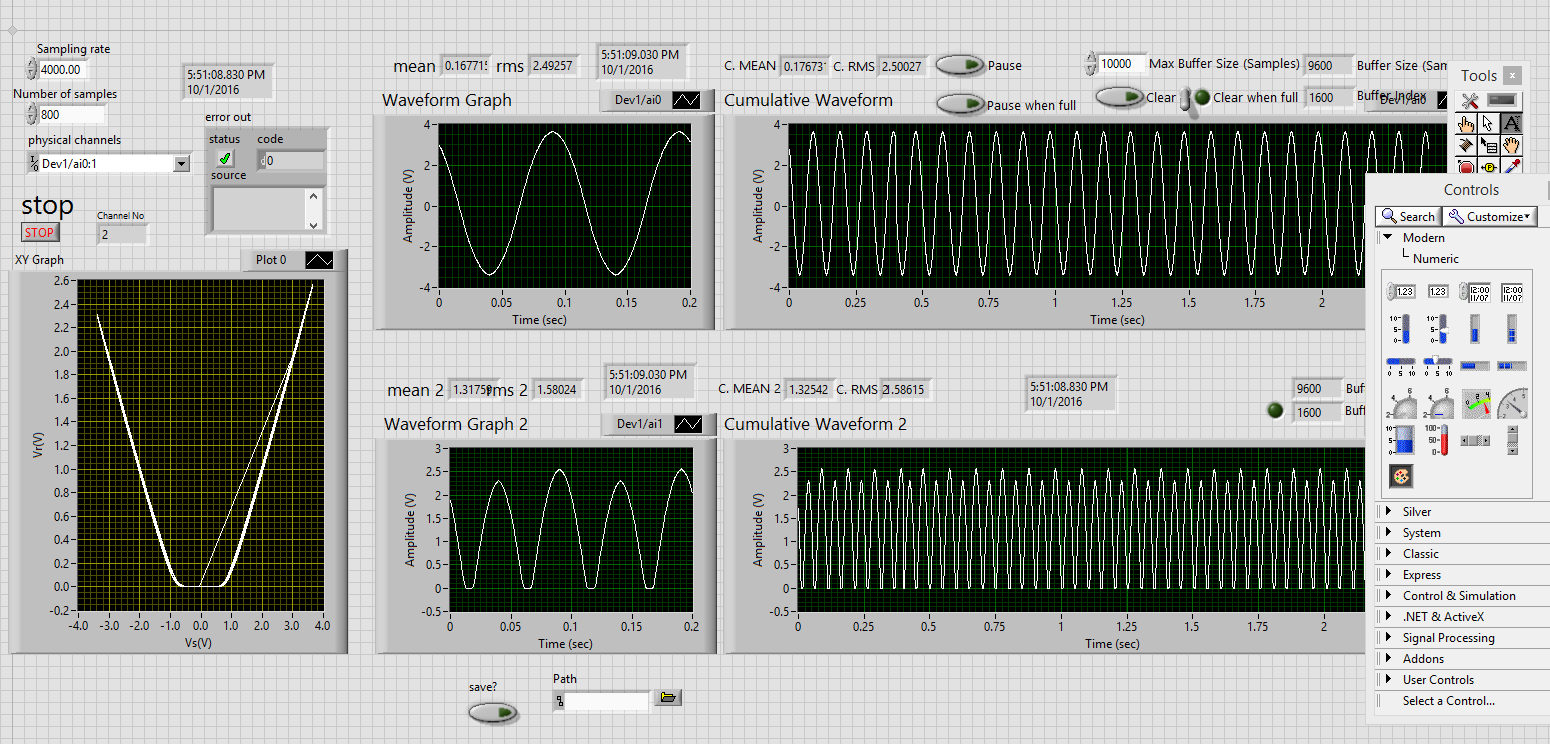
\includegraphics[width=\linewidth/1]{act5c10Hznocapac}
  \caption{The front panel of the full-wave rectifier without the capacitor(10Hz).}
  \label{fig:act5c10Hznocapac}
 \end{center}
\end{figure}



\end{document}
